\documentclass[11pt,a4paper]{article}
\usepackage[utf8]{inputenc}
\usepackage[T1]{fontenc}
\usepackage[francais]{babel}
\usepackage[fleqn]{amsmath}
\usepackage{amsfonts}
\usepackage{amssymb}
\usepackage{graphicx}
\usepackage{fullpage}
\usepackage{tikz}
\usepackage{algorithm}
\usepackage{algpseudocode}
\usepackage{enumitem}
\usepackage{slashbox}

\title{Algo avancée \\ Affectation \& Airport}

\newcommand{\second}{\prime\prime}

\begin{document}
	\maketitle
	
	\section{Affectation}
	\subsection{Énoncé}
	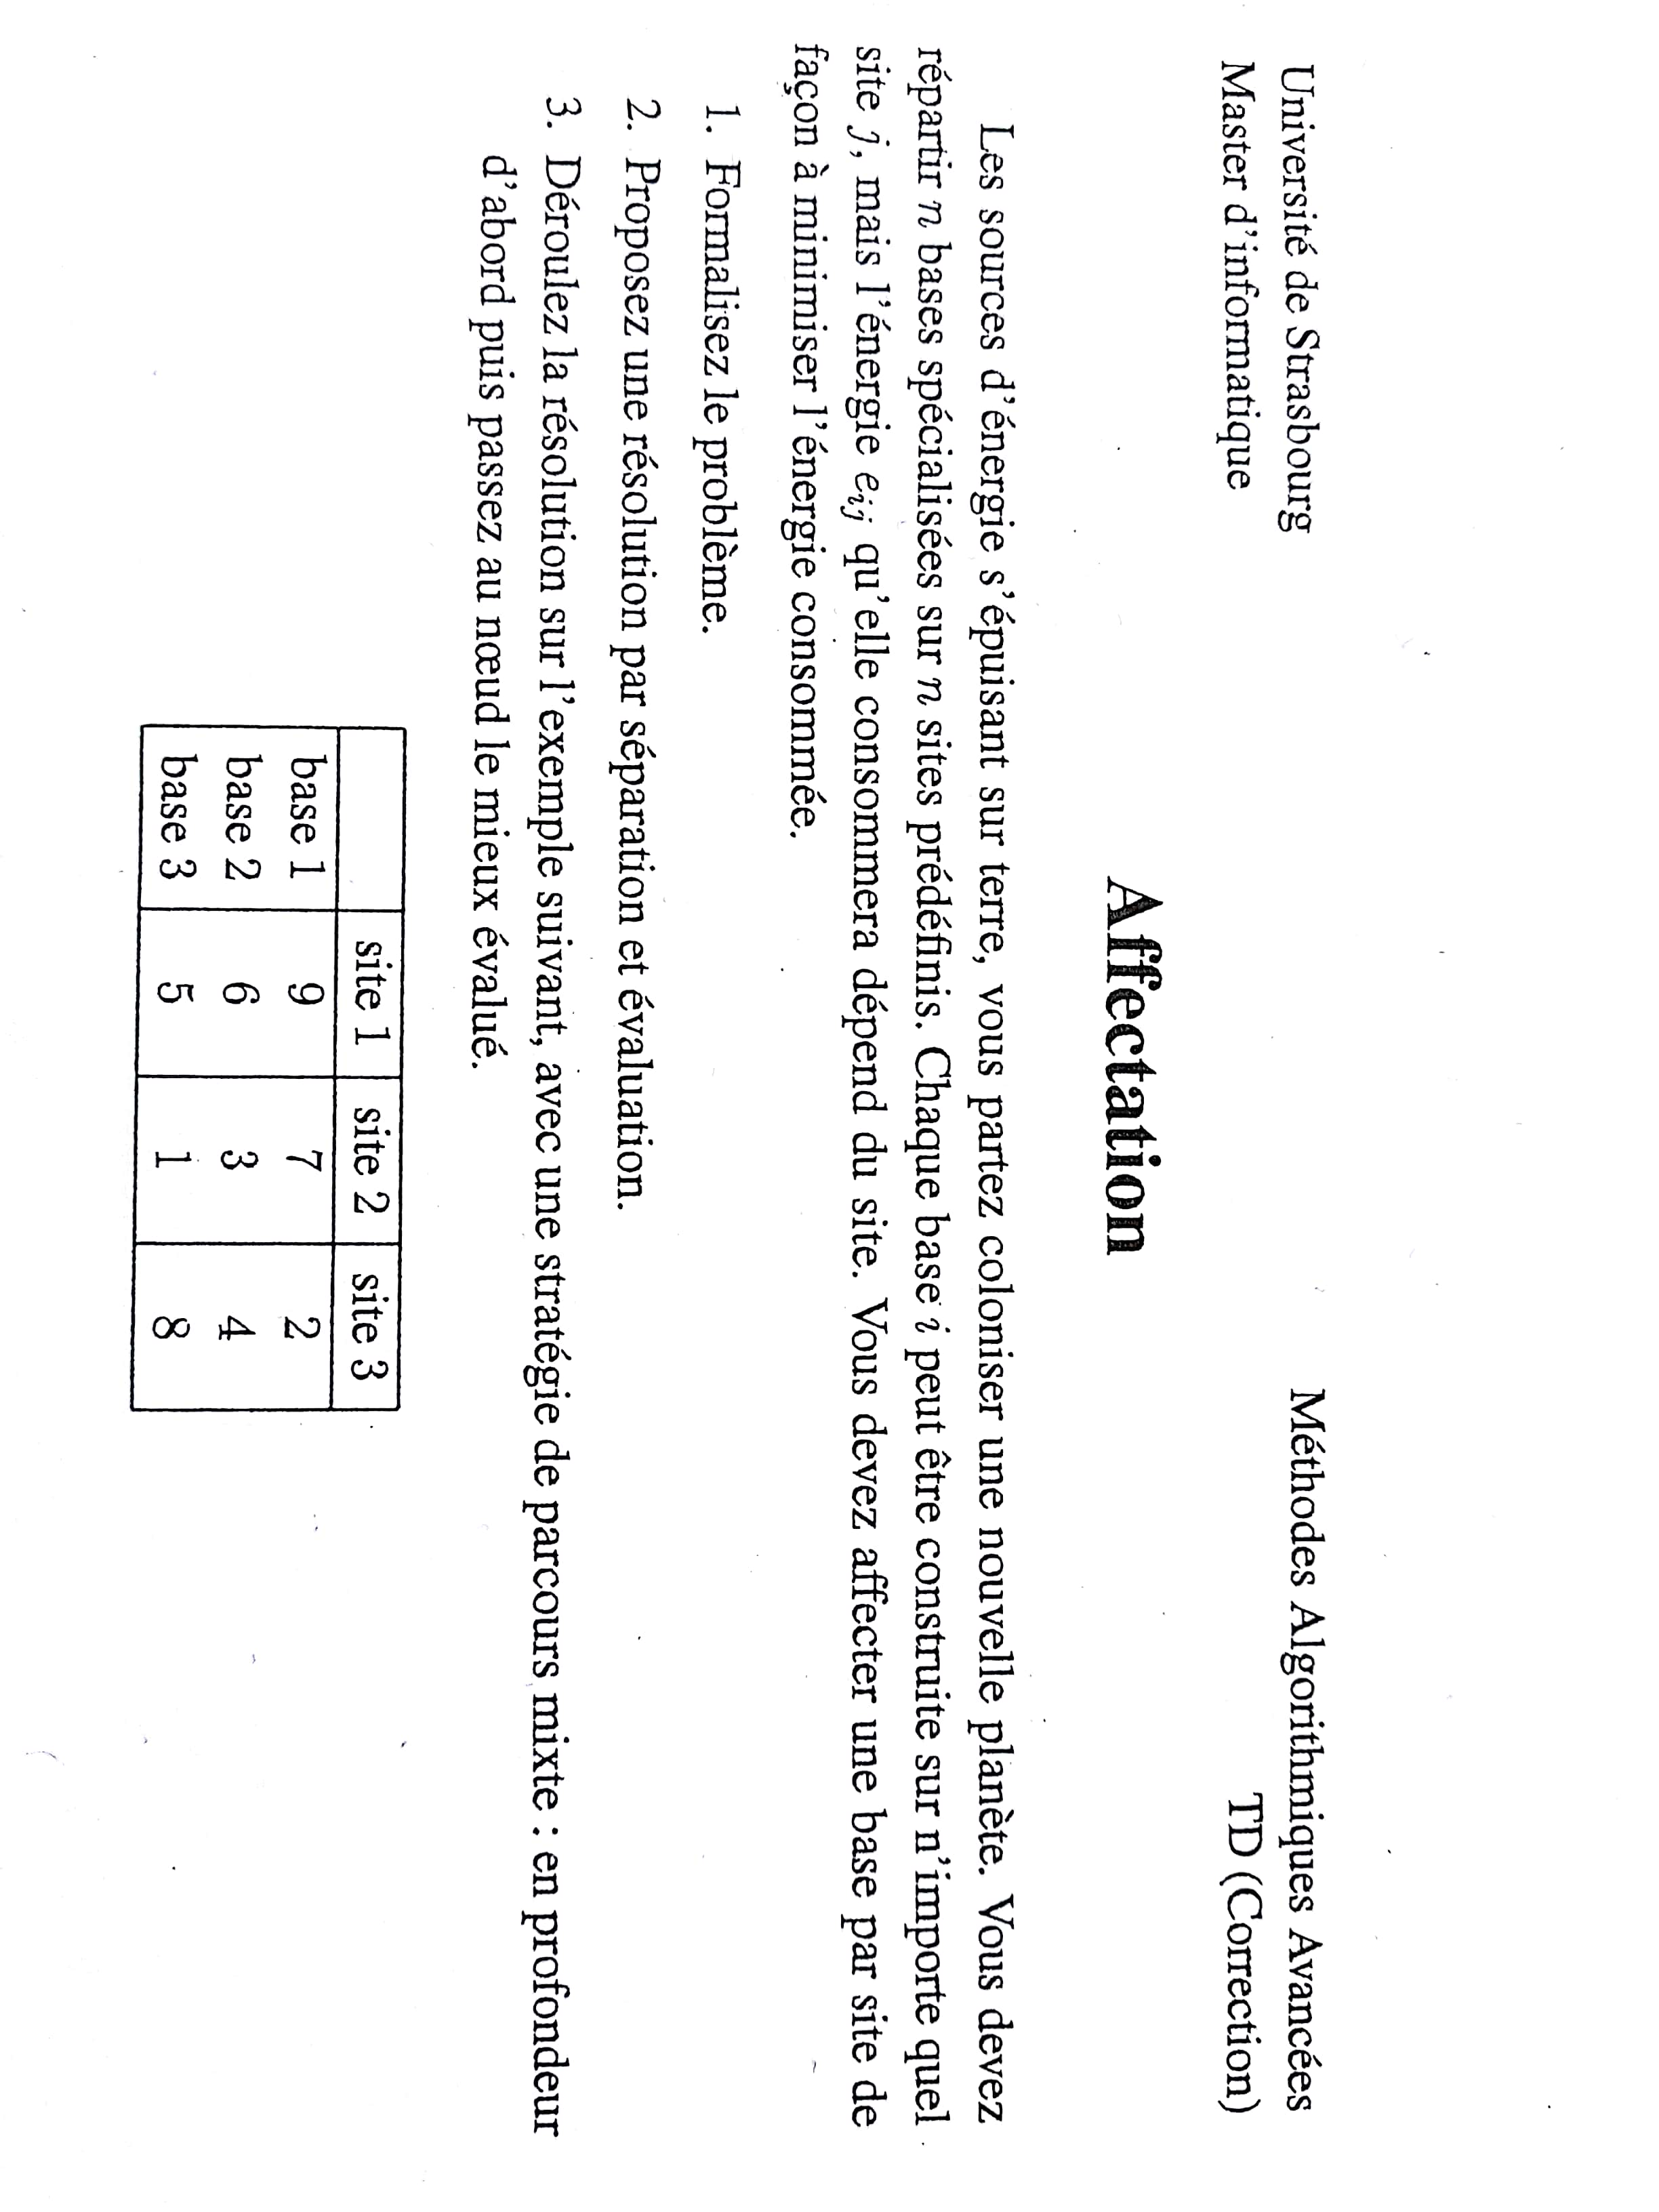
\includegraphics[angle=90,width=0.99\textwidth]{enonce.jpg}
	\newpage
	\subsection{Formalisation}
	\begin{itemize}
		\item n bases $1 \leqslant i \leqslant n$
		\item n sites $1 \leqslant j \leqslant n$
		\item $\rightarrow$ 1 base $\leftrightarrow$ 1 site, problème d'affectation $\Rightarrow$
 permutation de $[1,n]$
	\end{itemize}
	
	Une solution $S$ est permutation de $[1,n]\ \ S = \{j_i\},\ \ 1 \leqslant i \leqslant n$
	(La base i est affectée au site $j_i$)
	$$v(S) = \sum_{i=1}^{n} e_{i,j_{i}}$$
	$v(S)$ est la valeur d'une solution S. On veut minimum v(S). Niveau k permet de calculer $j_k$
	
	\subsection{Séparation et évaluation}
	\begin{itemize}
		\item noeud ? $S_k\ \text{donne} \{j_i\}, 1 \leqslant i \leqslant k$
		\item feuille ? $S_k\ \text{solutions}$
	\end{itemize}
	$$e(S_k) = \sum_{i=1}^{k} e_{i,j{i}} + \sum_{i=k+1}^{n} \underset{j \notin S_k}{min(e_{i,j{i}})}$$
	
	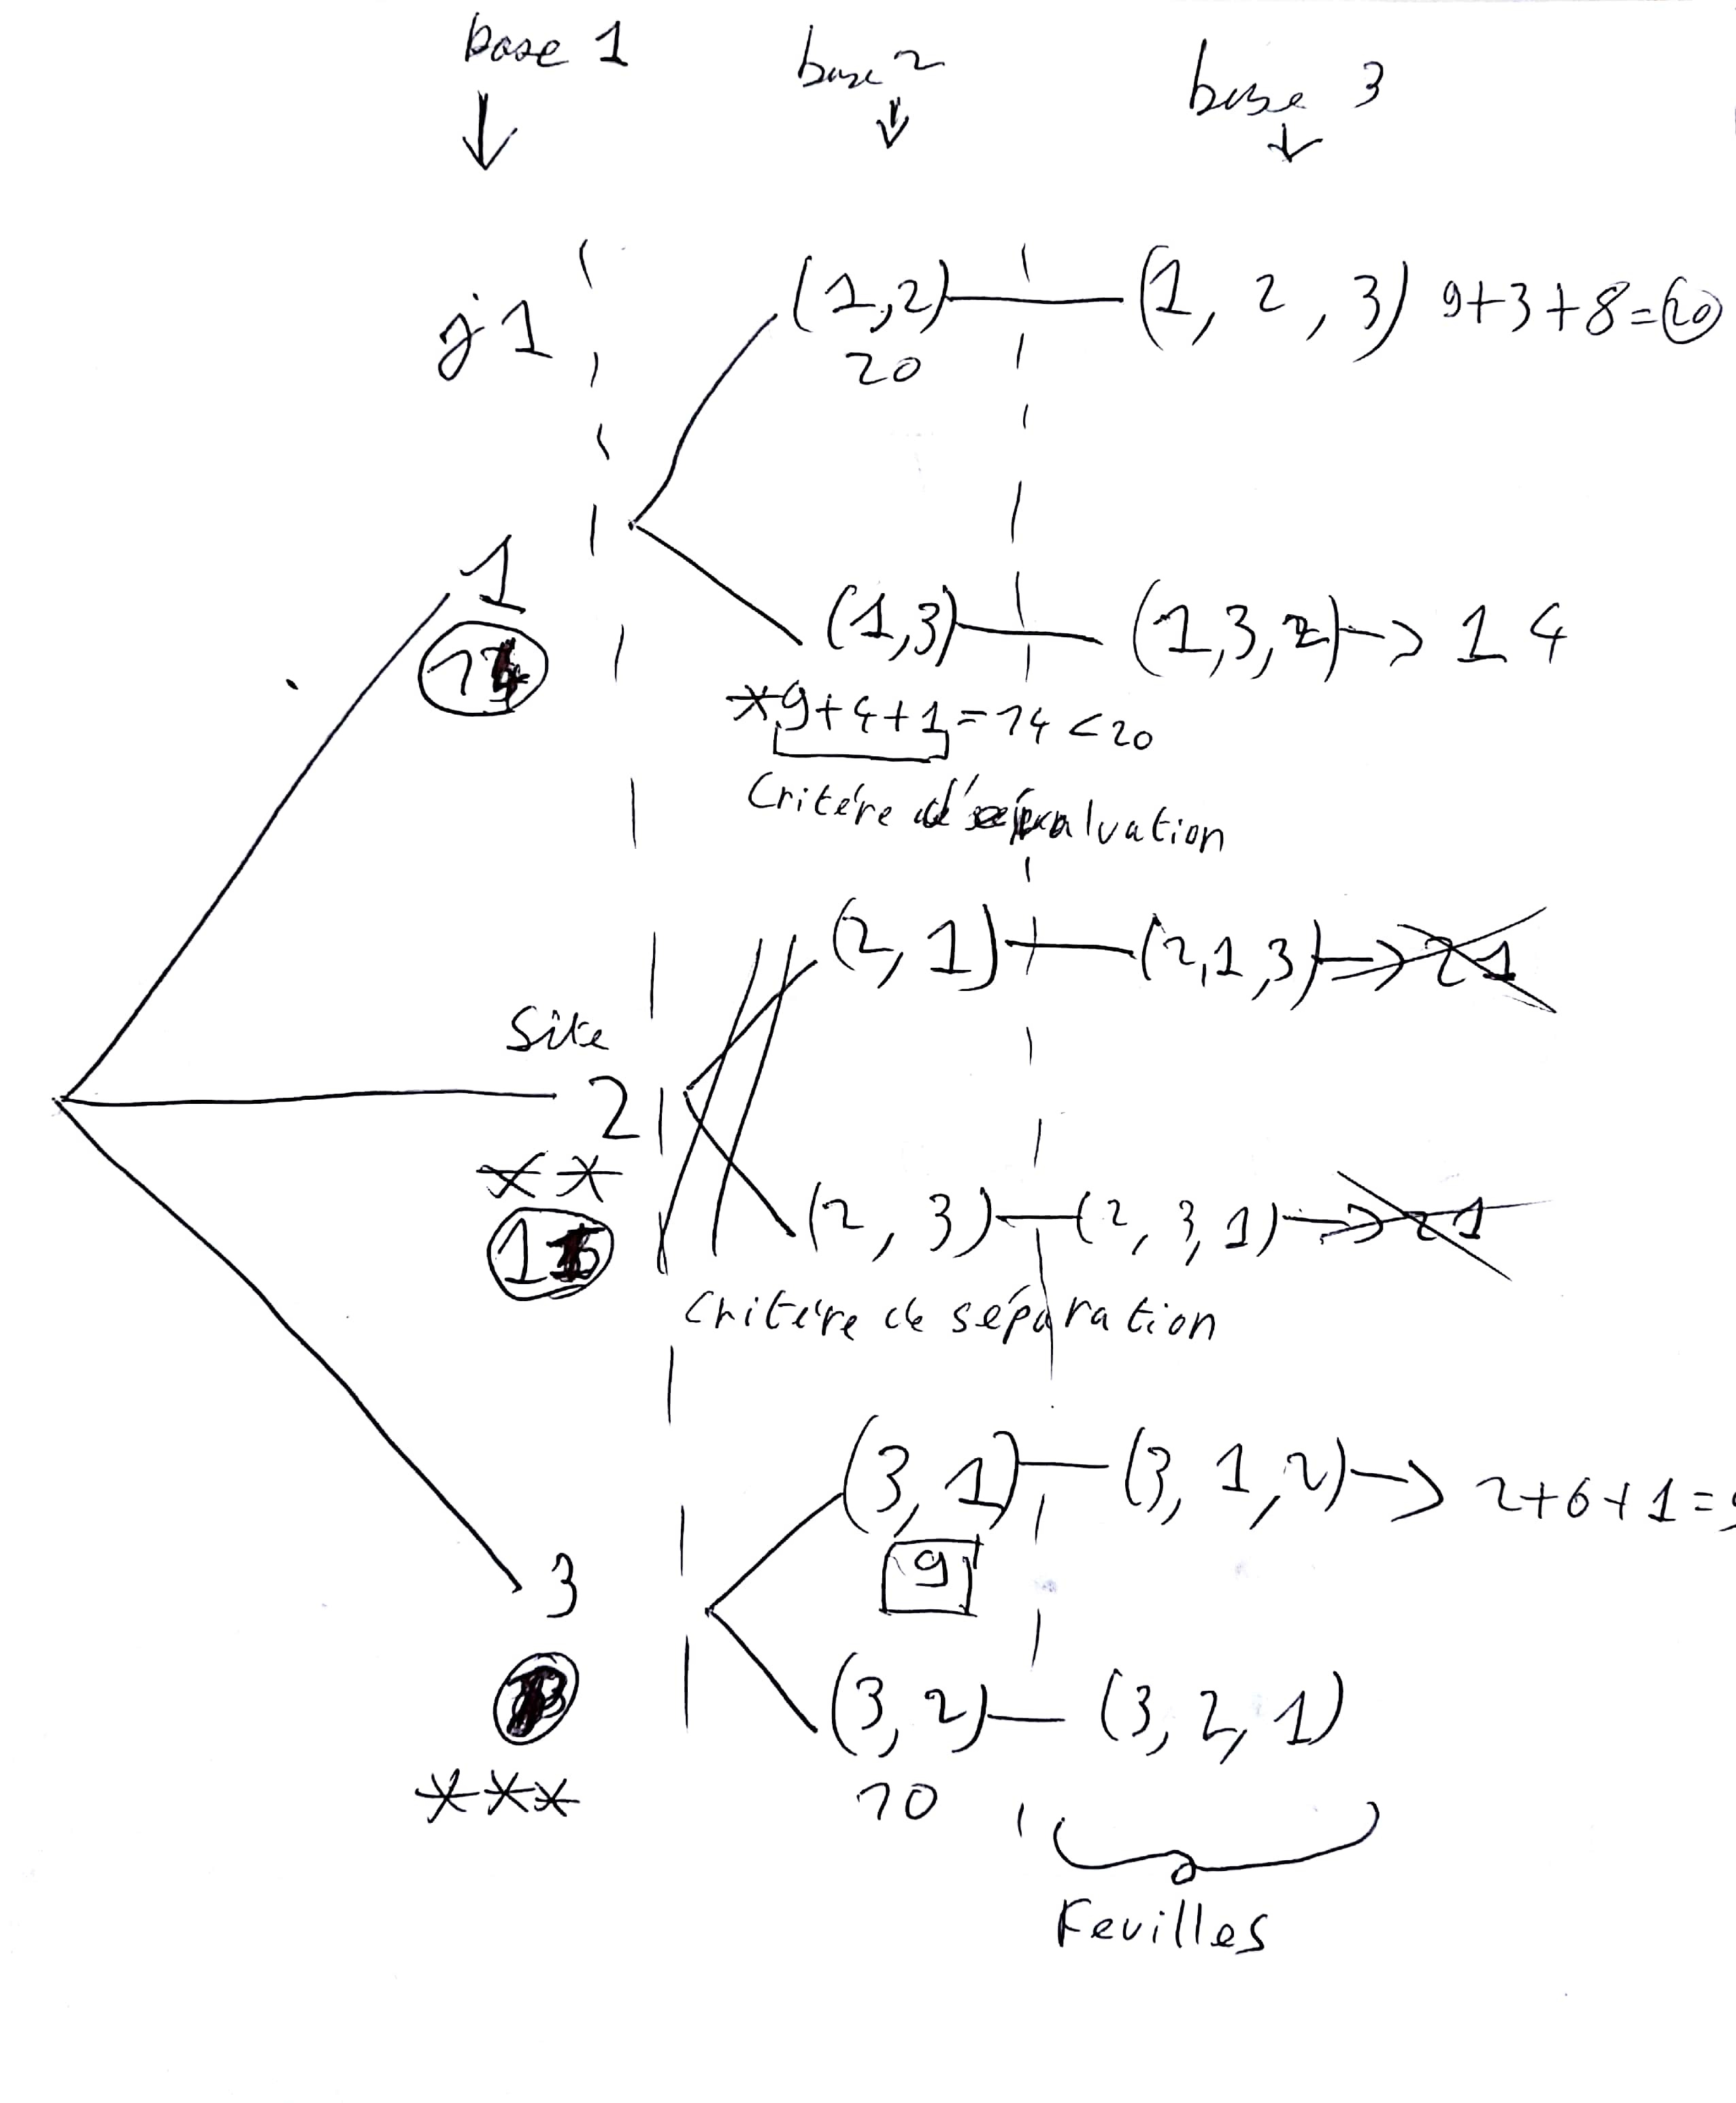
\includegraphics[width=0.93\textwidth]{arbre.jpg}
	
	\begin{itemize}
		\item * : $9 + 4 + min(1)$
		\item ** : $7 + min(6,5) + min(4,8) = 7 + 5 + 4 = 16$
		\item *** : $2 + min(6,5) + min(3,1) = 2 + 5 + 1 = 8$
	\end{itemize}
	\begin{center}
		\begin{tabular}{|c|c|c|c|}\hline
			\backslashbox{i}{j}&s1&s2&s3\\\hline
			b1&9&7&2\\\hline
			b2&6&3&4\\\hline
			b3&5&1&8\\\hline
		\end{tabular}
	\end{center}
	$$e(S_k) = \sum_{i=1}^{k} e_{i,j{i}} + \sum_{i=k+1}^{n} \underset{j \notin S_k}{min(e_{i,j{i}})}$$
	$$
	\begin{pmatrix} 
		i & 1 \\
		j_{1} & 2
	\end{pmatrix}\text{site 2 à la base 1}$$
	$e_{1,2} + min(6,4) + min(5,8) = 7 + 4 + 5 = 16$
	
	\section{Airport}
	\subsection{Énoncé}
	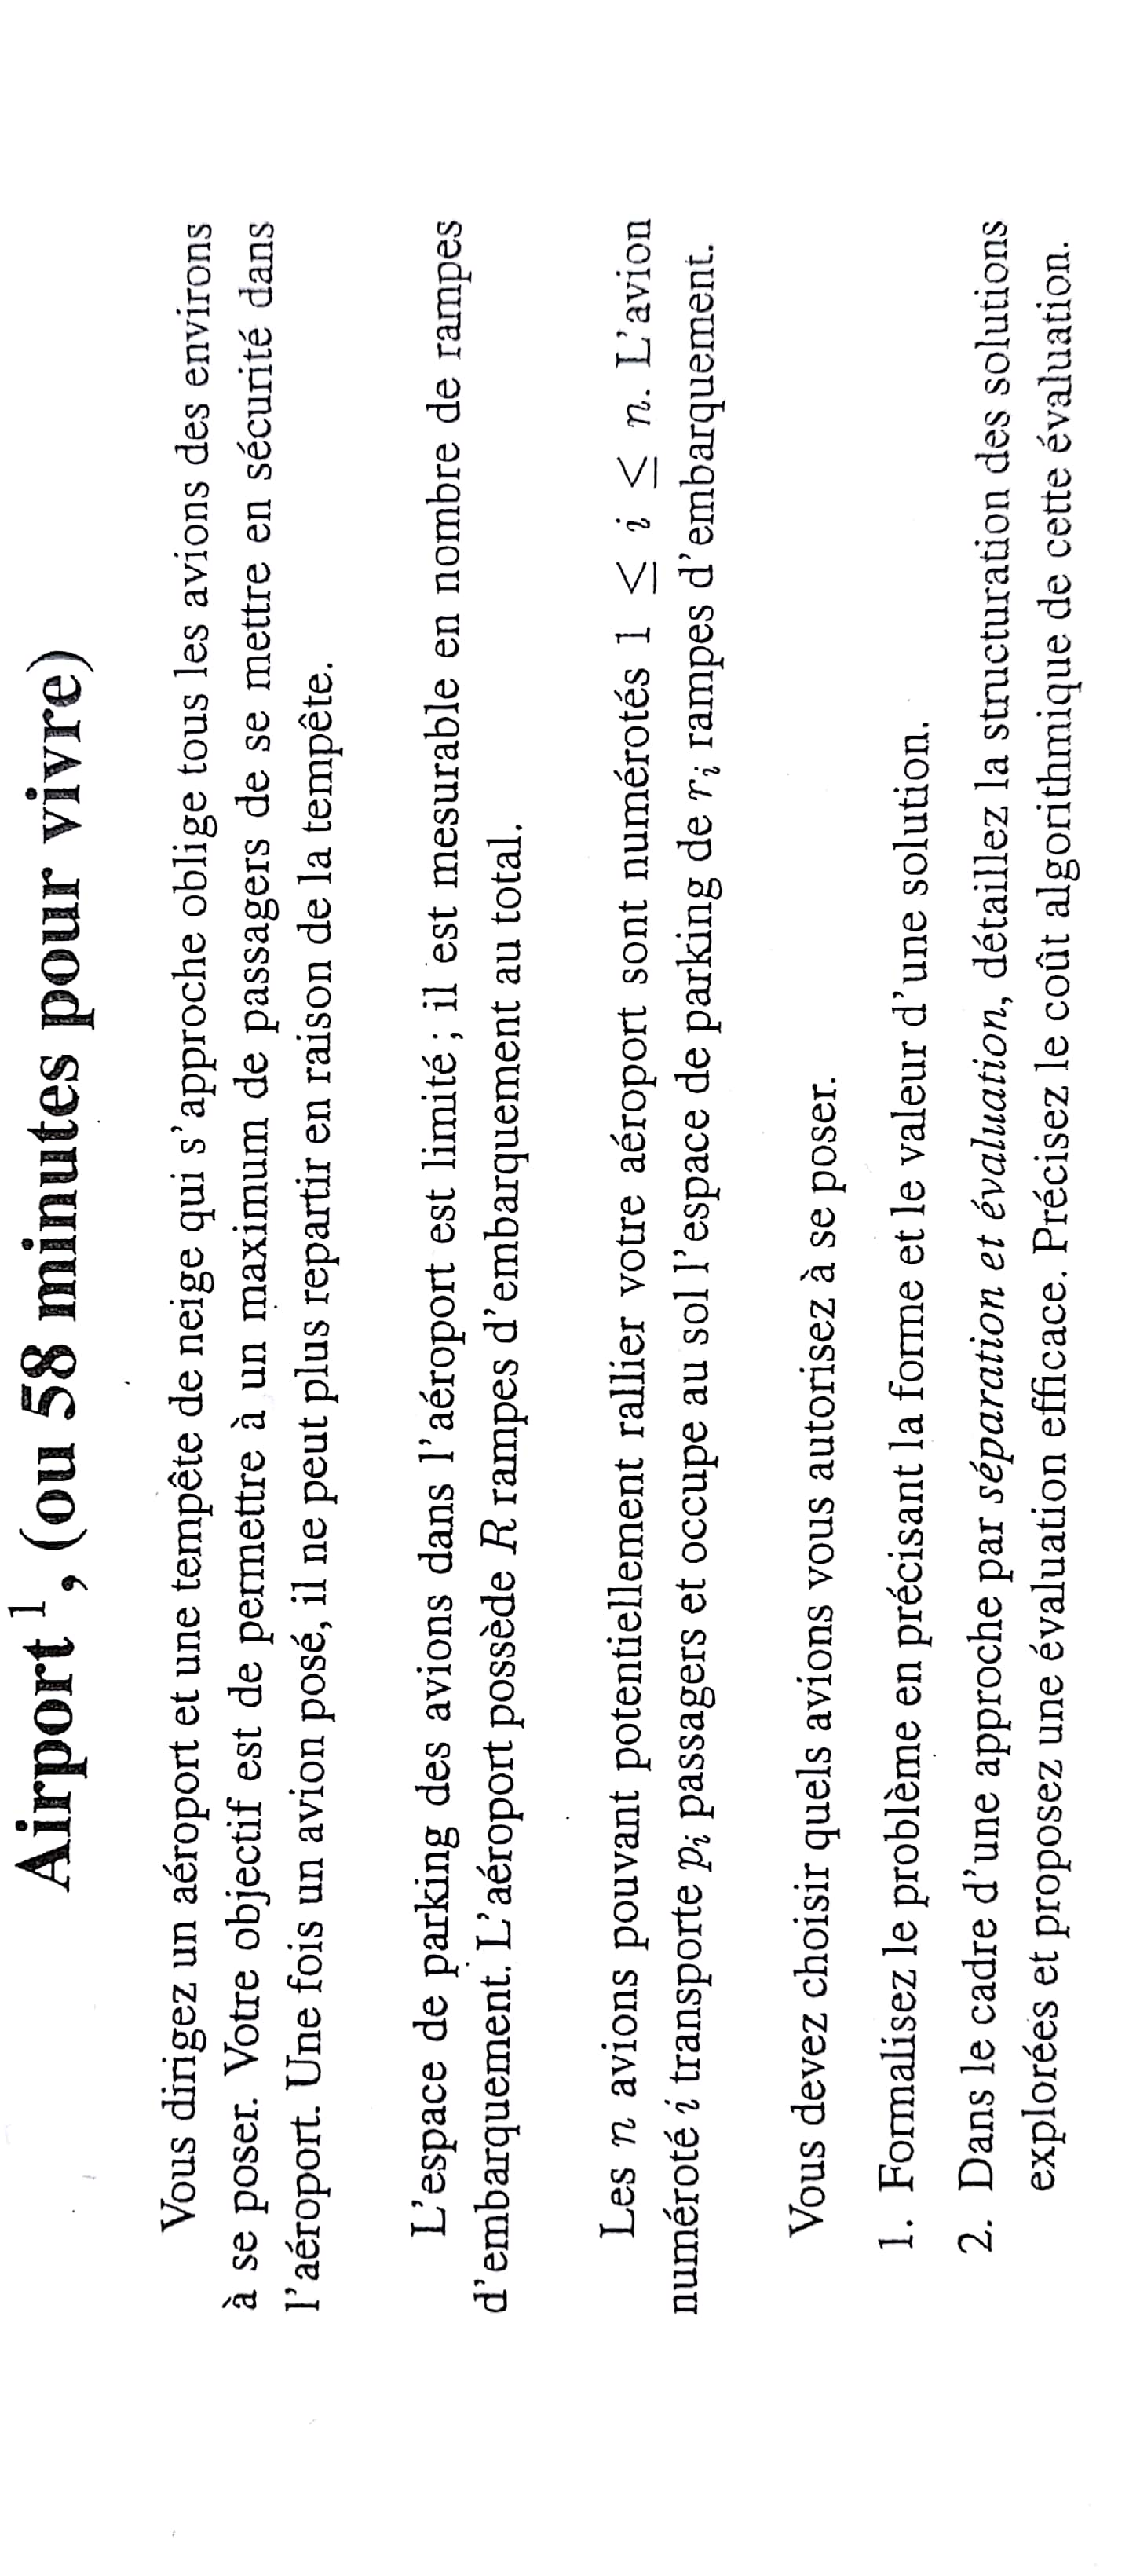
\includegraphics[angle=-90,width=0.99\textwidth]{airport.jpg}
	\newpage
	\subsection{Formalisation}
	\begin{itemize}
		\item n avions, $1 \leqslant i \leqslant n$
		\item Chaque avion i à $P_i$ passagers, occupe $r_i$ rampes
		\item $\rightarrow$ type "sac à dos"
		\item $\rightarrow$ chaque avion 1 seul fois
	\end{itemize}
	$$\text{La solution } S = \{b_1, b_2, b_3, ..., b_n\}$$
	$$b_i = {0,1}$$
	\begin{flalign*}
		\text{Critère d'admissibilité : }\Omega(S) &= \sum_{i=1}^{n} b_ir_i \leqslant R\\
		\text{Valeur d'une solution : }v(S) &= \sum_{i=1}^{n} b_ir_i
	\end{flalign*}
	
	$\Rightarrow$ On trie par ordre croissant les rapports $\frac{P_i}{r_i}$
	$$\frac{P_{\sigma(1)}}{r_{\sigma(1)}} \geqslant \frac{P_{\sigma(2)}}{r_{\sigma(2)}} \geqslant ... \geqslant \frac{P_{\sigma(n)}}{r_{\sigma(n)}}$$
	
	Le niveaux k permet de choisir $b_k$.
	
	$$
		\text{Noeud }S_k \begin{cases}
			e(S_k) = \sum_{i=1}^{k} b_{\sigma(i)}p_{\sigma(i)}\\
			r(S_k) = \sum_{i=1}^{k} b_{\sigma(i)}p_{\sigma(i)} \leqslant R
		\end{cases}
	$$
\end{document}